\chapter{Feature extraction} % (fold)
\label{chap:feature_extraction}
This chapters describes different approaches on the marker detection. It explains the trade-offs,methods that have been considered and applied for the different markers. The markers that have been analysed and detected in this project are Marker 1 (Color), Marker 2 (Thin lines) and Marker 3 (Corny). 

\begin{figure}[ht!]
	\centering
	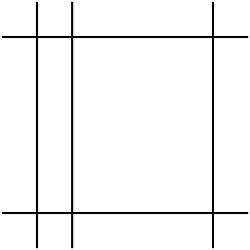
\includegraphics[width=100px]{figures/Marker2a}
	\caption{Marker 1 Color}
	\label{fig:markerColor}
\end{figure}


\section{Marker 1 (Color)} 
It is a trade-off between speed (how many detections per second) and precision (how precise the detection is). It is necessary to know whether a fast or a slowly moving object is being tracked. There are several options available. As more features are added to the code, runtime is likely to become longer. The runtime also depends on the computational capability of the computer.

Another trade-off lies in the universality of the detection - whether the detection is effective in a closed artificial environment (easier to detect) or in real "chaotic" environment (the simple methods may fail).

\newpage

Here goes first marker


\subsection{Center of mass}
For calculating the center of mass of the circles several options are available.
One possible solution is to calculate the centre of mass with use of the opencv function
moments() that calculates the moment of a contures and from these moment calculate the
center of mass. This is a very effective solution for calculating the center of mass of
objects with various shapes. This method seems to work perfectly for the easy and quite good
for the HARD sequence. Problem of this method occurs when detecting the marker in the hard sequence,
there sometimes the detected circle contours are not complete (luminosity differences) and the resulting
center of mass is shifted. 

The shapes that need to be detected have circle shapes. For this reason another less time-consuming 
method has been implemented. The center of mass is calculed with function minEnclosingCircle() whitch calculates
a surround circle for a given contour. When using this function the output circle center point is the
center of mass of the detected circle. this method improves the perfomance over the previously used 
moment method and the HARD sequence detection then proceeds without problems. This method can be improved 
with using approxPolyDP() before calling the minEnclosingCircle(). This functions approximates the contour
polygon and filles possible holes. Without approxPolyDP() the marker detection is faster.
\newpage
\section{Marker 2 (2a Thin lines)}

\newpage
\section{Marker 3 (Corny)}
% chapter featre_extraction (end)